
\documentclass{report}

\usepackage{tlatex}
\usepackage{listings}
\usepackage{xcolor}
\usepackage{comment}
\usepackage{fancyhdr}
\usepackage{amssymb}
\usepackage{inputenc}
\usepackage{svg}

\usepackage{tikz}
\usetikzlibrary{automata, positioning, arrows}


% !TeX spellcheck = en_GB 

% Configure fancyhdr
\pagestyle{fancy}
\fancyhf{} % Clear default header and footer

% Header settings
\fancyhead[L]{\nouppercase{\leftmark}} % Chapter number and title on the left
% \fancyhead[C]{Center Header}    % Centered header
\fancyhead[R]{\thepage}     % Right-aligned header

% Footer settings
% \fancyfoot[L]{Left Footer}      % Left-aligned footer
% \fancyfoot[C]{Page \thepage}    % Centered footer with page number
% \fancyfoot[R]{Right Footer}     % Right-aligned footer

% java -cp /home/richard/dev/tla2tex/tla2tools.jar  tla2tex.TeX  book.tex 

\lstset { %
    language=C++,
    backgroundcolor=\color{black!5}, % set backgroundcolor
    basicstyle=\footnotesize,% basic font setting
}

\title{Learning TLA+ by Examples}
\author{Richard Tang}
\date{\today}
\begin{document}
\maketitle
\tableofcontents

\chapter{Introduction}

\section{Catching Problems Early}

Years ago, I worked on a propietary low power processor in an embedded system.
The processor ran microcode featuring a custom instruction set. To enter a low
power state, a set of (possibly hundreds) instructions were executed. These
instructions progressively puts the system in lower power state. For example:
turn off IP A, then turn off IP B, then turn off the power island to the IPs. To
save cost and power, the low power processor had very limited debuggability
support.\newline

An experienced reader may start to notice some redflags.\newline

If the microcode attempts to access the memory interface when the power island
has been shut off, processor would hang. Since the power island has been shut
off, the physical hardware debug port is also shut off, leaving the developer
with \textit{no way} of live debugging related problem. At this point the
developer needs to siphon through (possibly hundreds) of instructions to catch
invariant violation \textit{manually}.\newline

As one can imagine, maintaining the microcode was very expensive for the team.
Fortunately, the propietary low power processor only had a handful of
instructions, I created an emulator for this propietary processor to verify the
microcode prior to deploying it on target. The emulator models the processor
states as a state graph, with executed instruction transitions the state machine
to to the next state. At every state all the invariants are evaluated to ensure
none have been violated. Examples of invariants included:
\begin{itemize}
    \item Accessing memory interface after power off leads to a hang
    \item Accessing certain register in certain chip revision leads to a hang 
    \item Verify IPs are shut off in the allowed order
\end{itemize}

The verification algorithm was implemented using a \textit{depth-first search}
algorithm, providing \textit{100\%} microcode coverage before deploy on
target.\newline

This was a very enlighting experience. To generalize, there are a class of
problem where the solution has high \textit{failure cost}. Solution such as
lockless or waitfree data structure, distributed algorithms, OS scheduler are
typically hard to reason about correctness because all the possible states
existed during execution. These solutions tend to have high failure cost because
related issues are difficult to reproduce and hard to debug. Good software
engineering practice suggest we need to implement tests, but tests do not cover
the entire state graph of the solution space exhaustively.\newline 

\textit{So, how do we ensure the solution is correct by design?}

\section{The Generalized Problem}

Fast forward to now: I stumbled across TLA+, a formalized solution of what I was
looking for.\newline

Leslie Lamport invented the TLA+ 1999, but TLA+ didn't appear to have caught on
until the 2010's. My personal opinion is TLA+ was invented ahead of its time,
and the problem complexity finally caught up in the past decade or so to allow
TLA+ to visibly demonstrate its strength.\newline

We are also at a point in the technology curve where vertical scaling is no
longer practical, with CPU speed plateau'd in the past decade or so. The
industry is exploring horizontal scaling solution, such as hardware vendor
focusing adding more CPU cores, or software vendors buying many low end hardware
instead of a few high end hardware. This shifts the technology complexity from
hardware to software, demanding software solution to maximize concurrent
hardware resource utilization. \newline

One slight problem: \textit{human are bad at concurrent reasoning.}\newline

Humans are fundamentally single-threaded machines. Reasoning things that execute
in parallel is possible, but difficult. It is hard to enumerate all possible
scenario in one's mind to ensure the design accommodates all the edge cases. 
\newline

Consider a distributed system. The system is a cluster of independently
operating entities and need to somehow collectively offer the correct system
behaviour, while any one of the machines may receive instructions out of order,
crash, recover, etc. \newline

Consider a single producer multiple consumer lockless queue. The consumers may 
reserve an index in the queue in certain order, but may release them in different order. 
What if one reader is really slow, and another reader is super fast and possibly 
lapse the slow reader? \newline

Consider an OS scheduler with locks. Assume all the processes have the same
priority. Can a process starve the other processes by repeatedly acquire and
release the lock? How do we ensure scheduling is fair?\newline

The usual \textit{anti-pattern} is to keep bandaiding the design until bugs stop
comming. This is never ideal. Per Murphy's law, anything that can go wrong will
go wrong, and a hard to reproduce bug will come in at the most inconvinient
time. How do we make sure the solution is actually \textit{correct by design}?
To solve this problem, we must rely on tools to do the reasoning \textit{for
us}.

\section{TLA+}

TLA+ is a \textit{system specification language}, with the intent to describe
the system with implementation details removed. TLA+ allows designer to describe
the system as a sequence of states. The designer can expresses transition
condition from one state to another, describe invariants that must hold true in
every state and liveness properties that the overall system should converge to.
The key innovation of TLA+ is once the system is modeled as a finite state
machine, the states can be \textit{exhaustively} explored (via
breath-first-search) to ensure certain properties are held through out the
entire state space (either per state or a sequence of states).\newline

\section{Target Audience}

The intent for the book is to teach reader how to write TLA+ spec for their
design to provide confidence in \textit{design correctness}. The content to this
book is appropriate for software designer, hardware designer, system architect,
and such.\newline 

As for the readers: some computing science knowledge is required. One doesn't
need to be expert at a particular language to understand this book; TLA+ is
effectively its own language. This book is example driven and will go through
designs such as lockless queue, simple task scheduler, consensus algorithm, etc.
Reader will likely enjoy a deeper insight if she has some familiarity with these
topics.

\section{Book Layout}

This book was motivated by the intent to solve problems. The book is designed to
be example heavy with many chapter each represnting an problem that can be
modelled using TLA+.\newline

Examples are split into two categories: A set of examples written using native
TLA+ syntax, and another set of examples written using PlusCal (C-like syntax).
I believe they are useful under different use cases. The differences will be
highlighted in their respective sections. All examples will follow a similar 
layout, covering the expected design process (eg. requirement, spec, safety and
liveness properties). \newline

Finally, there will be part that language reference portion that that discuss a
few topics deserving extra attention. The intent is to be using this section of the 
book as a \textit{reference}.

\chapter{TLA+ Primer}

\section{Design Intent}

The key insight into TLA+ is modelling a system as a state machine. A blinking
LED system can be described using a single variable with two states, LED being
on or off. A simple digital clock can be represented by two variables, hour and
minute and the number of possible states in a digital clock is $24 * 60 = 1440$.
For example, 10:01 is the next state 10:00 can transition to.  Extrapolating
further, Asssume an arbitrarily system described by N variables, each variable
having K possible values such arbitrary system can have up to $N^K$
state.\newline

For every specification, designer can specify \textit{safety} proerty (or
invariants) that must be true in \textit{every} states. For example, in any
state of the digital clock hour \textit{must} be between 0 to 23, or formally
described as $hour \in 0..23$.  Similarly, $minute \in 0..59$. More generic
invariant examples include: in any state, only one thread has exclusive access
to a critical region, all variables in the system are within allowable value,
the resource allocation manager never allocates more than available resources,
etc. \newline

Designer can also specify \textit{liveness} property. These are properties that
are satisfied by a \textit{sequence of state}. One liveness property for the
digital clock could be when the clock is $10:00$, it will eventually become
$11:00$ (\textit{$10:00$ leads to $11:00$}). More generic liveness property
include: a distributed system eventually converges, the scheduler eventually
schedules every tasks in the task queue, the resource allocation manager fairly
allocates resources, etc. \newline

TLC checks a TLA+ spec using \textit{breath-first search} algorithm to explore
\textit{all} states in the state machine and ensure safety and liveness
properties are upheld. TLA+ specifies the system using \textit{propositional
logic}. 

\section{Requirement}

In this example, we will specify a \textit{digital clock}. The digital clock has
a few simple requirements:
\begin{itemize}
    \item Two variables to represent state: hour and minute
    \item The clock increment one minute at a time
    \item The clock wraps around at midnight (ie. 23:59 transitions to 00:00)
\end{itemize}

\section{Spec}

The \textit{Init} state of such system can be described as: \newline
\begin{tla}
    Init ==
        /\ hour = 0
        /\ minute = 0
\end{tla}
\begin{tlatex}
\@x{\@s{16.4} Init \.{\defeq}}%
\@x{\@s{32.8} \.{\land} hour \.{=} 0}%
\@x{\@s{32.8} \.{\land} minute \.{=} 0}%
\end{tlatex}
 \newline

$\defeq$ is the \textit{defines equal} symbol and $\land$ is the \textit{logical
and} symbol. The above TLA+ syntax can be read as \textit{Init} state is defined
as both hour and minute are both 0.\newline

The spec also always include a $Next$ definition, an \textit{action formula}
describing how the system transition from one state to another. Action formula
contains \textit{primed} variables what happens to the variable in its next
state. The $Next$ action for the digital clock can be defined as:\newline

\begin{tla}
    NextHour ==
        /\ minute = 59 
        /\ hour' = (hour + 1) % 24
        /\ minute' = 0
    NextMinute == 
        /\ minute # 59
        /\ hour' = hour 
        /\ minute' = minute + 1 
    Next ==
        \/ NextMinute
        \/ NextHour
\end{tla}
\begin{tlatex}
\@x{\@s{16.4} NextHour \.{\defeq}}%
\@x{\@s{32.8} \.{\land} minute \.{=} 59}%
\@x{\@s{32.8} \.{\land} hour \.{'} \.{=} ( hour \.{+} 1 ) \.{\%} 24}%
\@x{\@s{32.8} \.{\land} minute \.{'} \.{=} 0}%
\@x{\@s{16.4} NextMinute \.{\defeq}}%
\@x{\@s{32.8} \.{\land} minute \.{\neq} 59}%
\@x{\@s{32.8} \.{\land} hour \.{'} \.{=} hour}%
\@x{\@s{32.8} \.{\land} minute \.{'} \.{=} minute \.{+} 1}%
\@x{\@s{16.4} Next \.{\defeq}}%
\@x{\@s{32.8} \.{\lor} NextMinute}%
\@x{\@s{32.8} \.{\lor} NextHour}%
\end{tlatex}
 \newline

Here's a breakdown of what the spec does:
\begin{itemize}
    \item $Next$ can take $NextMinute$ or $NextHour$
    \item $Next$ takes $NextMinute$ when $minute$ is not 59, next hour is hour, next minute is minute + 1. 
    \item $Next$ takes $NextHour$ when $minute$ is 59, next hour is (hour + 1) modulus 24, next minute set to 0
\end{itemize}

Technically it's possible for $Next$ to take both $NextMinute$ and $NextHour$.
This is not possible in this definition as $NextHour$ and $NextMinute$ are
defined in a \textit{mutually exlusively} fashion.\newline

Finally, the spec itself is formally defined as:\newline
\begin{tla}
    vars == <<hour, minute>>
    Spec ==
        /\ Init
        /\ [][Next]_vars
\end{tla}
\begin{tlatex}
\@x{\@s{16.4} vars\@s{0.63} \.{\defeq} {\langle} hour ,\, minute {\rangle}}%
\@x{\@s{16.4} Spec \.{\defeq}}%
\@x{\@s{32.8} \.{\land} Init}%
\@x{\@s{32.8} \.{\land} {\Box} [ Next ]_{ vars}}%
\end{tlatex}
\newline

$\Box[Next]_{vars}$ deserves some special attention:
\begin{itemize}
    \item $vars$ is defined to be \textit{all} variables in the spec. Different
    combination of these variables constitute the states of the system (eg.
    23:59 and 00:00 are both states in the system).
    \item $\Box[Next]_{vars}$ is a \textit{box-action formula}, where
    \textit{Next} is an action and \textit{vars} is a state function.
    \item $\Box$ operator asserts the formula is always true for every step in the behaviour.
    \item And steps in the behaviour is defined as $[Next]_{vars}$, where $Next$
    describe the action and $vars$ capturing all variables representing the state.
\end{itemize}

%  $,  The formula is true iff every
% successive pair of steps in behaviour is a $[Next]_{vars}$. Finally $Spec$ is
% conjunction between $Init$ and $\Box[Next]_{vars}$. Note \textbf{all} TLA+
% specification follows very similar template. There are situation we will need to
% provide \textit{fairness} description - this will be covered later. \newline

\section{Safety}

Safety property describes invariant that must hold true in every state of
system. A common invariant is \textit{type safety} checks. In a digital clock, 
hour can only be in value between 0 to 23, and minute can only be value of 0 to 59:\newline

\begin{tla}
    Type_OK == 
        /\ hour \in 0..23
        /\ minute \in 0..59
\end{tla}
\begin{tlatex}
\@x{\@s{16.4} Type\_OK \.{\defeq}}%
\@x{\@s{32.8} \.{\land} hour \.{\in} 0 \.{\dotdot} 23}%
\@x{\@s{32.8} \.{\land} minute \.{\in} 0 \.{\dotdot} 59}%
\end{tlatex}

\section{Liveness}

Liveness property verifies certain behavioural across a sequence of state. One
liveness property can be confirming the clock wraps around correctly at
midnight (which involves mutliple states): \newline

\begin{tla}
    Liveness ==
        /\ hour = 23 /\ minute = 59 ~> hour = 0 /\ minute = 0
\end{tla}
\begin{tlatex}
\@x{\@s{16.4} Liveness \.{\defeq}}%
 \@x{\@s{32.8} \.{\land} hour \.{=} 23 \.{\land} minute \.{=} 59 \.{\leadsto}
 hour \.{=} 0 \.{\land} minute \.{=} 0}%
\end{tlatex}
\newline

$\leadsto$ is the \textit{leads to} operator, suggesting something is eventually
true. TLA+ provides a set of formulas that can be used to describe liveness
property.\newline 

To verify liveness, we need to modify the spec slightly to enable
\textit{fairness} to prevent \textit{stuttering}. In plain terms, fairness
ensure \textit{something} always happen in every step, allowing the states to
transition. Without fairness the spec is allowed to \textit{do nothing} as next
step, this means liveness condition may fail because the spec permits the system
to do nothing in perpetuity as next state. Fairness will be covered in more
detailed in later chapter.\newline

\begin{tla}
    Spec ==
        /\ Init
        /\ [][Next]_vars
        /\ WF_vars(Next)
\end{tla}
\begin{tlatex}
\@x{\@s{16.4} Spec \.{\defeq}}%
\@x{\@s{32.8} \.{\land} Init}%
\@x{\@s{32.8} \.{\land} {\Box} [ Next ]_{ vars}}%
\@x{\@s{32.8} \.{\land} {\WF}_{ vars} ( Next )}%
\end{tlatex}
\newline

$WF_{vars}(Next)$ is the fairness qualifier.

% TODO: insert reference here to specifying systems 8.1 

\section{Model Checker}

The TLA+ spec can be verified using TLC model checker. The TLC model checker
runs the spec and verifies all configured safety and liveness properties are
satisfied during execution. To run TLC, we need two things:
\begin{itemize}
    \item clock.tla - the spec itself
    \item clock.cfg - the corresponding configuration file
\end{itemize}

For reference, clock.tla spec is listed below:

\begin{tla}
--------------------------- MODULE clock ----------------------------
EXTENDS Naturals
VARIABLES hour, minute
vars == <<hour, minute>>
Type_OK == 
    /\ hour \in 0..23
    /\ minute \in 0..59
Liveness ==
    /\ hour = 23 /\ minute = 59 ~> hour = 0 /\ minute = 0
Init ==
    /\ hour = 0
    /\ minute = 0
NextMinute ==
    /\ minute = 59 
    /\ hour' = (hour + 1) % 24
    /\ minute' = 0
NextHour == 
    /\ minute # 59
    /\ hour' = hour 
    /\ minute' = minute + 1 
Next ==
    \/ NextMinute
    \/ NextHour
Spec ==
  /\ Init
  /\ [][Next]_vars
  /\ WF_vars(Next)
=============================================================================
\end{tla}
\begin{tlatex}
\@x{}\moduleLeftDash\@xx{ {\MODULE} clock}\moduleRightDash\@xx{}%
\@x{ {\EXTENDS} Naturals}%
\@x{ {\VARIABLES} hour ,\, minute}%
\@x{ vars \.{\defeq} {\langle} hour ,\, minute {\rangle}}%
\@x{ Type\_OK \.{\defeq}}%
\@x{\@s{16.4} \.{\land} hour \.{\in} 0 \.{\dotdot} 23}%
\@x{\@s{16.4} \.{\land} minute \.{\in} 0 \.{\dotdot} 59}%
\@x{ Liveness \.{\defeq}}%
 \@x{\@s{16.4} \.{\land} hour \.{=} 23 \.{\land} minute \.{=} 59 \.{\leadsto}
 hour \.{=} 0 \.{\land} minute \.{=} 0}%
\@x{ Init \.{\defeq}}%
\@x{\@s{16.4} \.{\land} hour \.{=} 0}%
\@x{\@s{16.4} \.{\land} minute \.{=} 0}%
\@x{ NextMinute \.{\defeq}}%
\@x{\@s{16.4} \.{\land} minute \.{=} 59}%
\@x{\@s{16.4} \.{\land} hour \.{'} \.{=} ( hour \.{+} 1 ) \.{\%} 24}%
\@x{\@s{16.4} \.{\land} minute \.{'} \.{=} 0}%
\@x{ NextHour \.{\defeq}}%
\@x{\@s{16.4} \.{\land} minute \.{\neq} 59}%
\@x{\@s{16.4} \.{\land} hour \.{'} \.{=} hour}%
\@x{\@s{16.4} \.{\land} minute \.{'} \.{=} minute \.{+} 1}%
\@x{ Next \.{\defeq}}%
\@x{\@s{16.4} \.{\lor} NextMinute}%
\@x{\@s{16.4} \.{\lor} NextHour}%
\@x{ Spec \.{\defeq}}%
\@x{\@s{8.2} \.{\land}\@s{0.16} Init}%
\@x{\@s{8.2} \.{\land}\@s{0.16} {\Box} [ Next ]_{ vars}}%
\@x{\@s{8.2} \.{\land}\@s{0.16} {\WF}_{ vars} ( Next )}%
\@x{}\bottombar\@xx{}%
\end{tlatex}

The corresponding clock.cfg is listed below: 
\begin{lstlisting}
    SPECIFICATION Spec
    INVARIANTS Type_OK
    PROPERTIES Liveness
\end{lstlisting}

Now run TLC and one should see something like this: 
\begin{lstlisting}
Model checking completed. No error has been found.
...
The depth of the complete state graph search is 1440.
\end{lstlisting}

\part{Examples}

\chapter{Blinking LED}

Let's start with a trivial specification of a blinking LED. The intent of this example 
is to demonstrate the core functionalities of TLA+ specification language.

TODO: briefly talk about tla+ and model checker here.

\section{Requirement}

The LED is represented by a boolean variable that can be either 0 or 1.\newline

... that's it.

\section{Spec}

The specification language may appear alienating as it is mathematically
motivated based on propositional logic. Despite the (possibly) daunting syntax,
designer only need to be familiar with a handful of key operators to start
realizing value using TLA+. This chapter will attempt to describe the example in
exhaustive detail to reduce the learning curve.

The following describe the core portion of the blinking LED spec. 

\begin{tla}
--------------------------- MODULE blinking ----------------------------
VARIABLES b 
vars == <<b>>
Init ==
    /\ b = 0
On == 
    /\ b = 0
    /\ b' = 1
Off == 
    /\ b = 1
    /\ b' = 0
Next ==
    \/ Off 
    \/ On
Spec ==
    /\ Init
    /\ [][Next]_vars
========
\end{tla}
\begin{tlatex}
\@x{}\moduleLeftDash\@xx{ {\MODULE} blinking}\moduleRightDash\@xx{}%
\@x{ {\VARIABLES} b}%
\@x{ vars \.{\defeq} {\langle} b {\rangle}}%
\@x{ Init\@s{2.02} \.{\defeq}}%
\@x{\@s{16.4} \.{\land} b \.{=} 0}%
\@x{ On \.{\defeq}}%
\@x{\@s{18.15} \.{\land} b \.{=} 0}%
\@x{\@s{18.15} \.{\land} b \.{'} \.{=} 1}%
\@x{ Off \.{\defeq}}%
\@x{\@s{15.91} \.{\land} b \.{=} 1}%
\@x{\@s{15.91} \.{\land} b \.{'} \.{=} 0}%
\@x{ Next \.{\defeq}}%
\@x{\@s{16.4} \.{\lor} Off}%
\@x{\@s{16.4} \.{\lor} On}%
\@x{ Spec \.{\defeq}}%
\@x{\@s{16.4} \.{\land} Init}%
\@x{\@s{16.4} \.{\land} {\Box} [ Next ]_{ vars}}%
\@x{}\bottombar\@xx{}%
\end{tlatex}

\begin{itemize}
    \item $\defeq$ is the \textit{defines equal} operator 
    \item $\land$ and $\lor$ are the AND and OR operator. The effect
    of these operator follow the natural definition in English: 
    \begin{itemize}
        \item $C \defeq A \land B$: C is true iff A and B are true
        \item $C \defeq A \lor B$: C is true iff A or B is true
    \end{itemize}
    \item The $'$ operator represents the next state. $b'$ represent b's next state. 
    \item $VARIABLES$ keyword defines a list of variables for the spec. In this case 
    the spec defines a variable $b$ which can be either 0 or 1
    \item $vars$ is typically defined as a shorthand to refer to \textit{all}
    variables in the spec. 
\end{itemize}

With the above definition, we can revisit the Action definitions: $Init$ defines
the initial system state, where b is set to 0.\newline 

$Next$ requires more elaboration. TLA+ specifies the system as a collection of
states with transitions between them. In a simplified sense, the state is
described as a collection of ANDs (eg. system is in state C if both A and B are
true), the ORs then describe the states the system can possibly be in (eg.
system can be in state C OR D). Revisiting the example, the blinking LED has two
states:
\begin{itemize}
    \item $On \defeq b = 0 \land b' = 1$: b switches on 
    \item $Off \defeq = 1 \land b' = 0$: b switches off
\end{itemize}

The system's $Next$ state is defined to be one of these states:\newline
$Next \defeq On \lor Off$.\newline

$\Box[Next]_{vars}$ is a \textbf{Box-Action Formula}, where \textit{Next} is an
action and \textit{vars} is a state function. The formula is true iff every
successive pair of steps in behaviour is a $[Next]_{vars}$. Finally $Spec$ is
conjunction between $Init$ and $\Box[Next]_{vars}$. Note \textbf{all} TLA+
specification follows very similar template. There are situation we will need to
provide \textit{fairness} description - this will be covered later. \newline

In short: this specification describes a two-state state machine where b toggles
between 0 and 1.\newline

Note that b can technically be \textit{anything}. b can be 0, 1, -42, a
dinosaur, etc. TLA+ specifies values of $b$ which are valid in the system.

\section{Safety}

The spec so far only defines the possible states - but the \textit{power} of
TLA+ lies in its \textit{properties} description. Safety properties are
invariants that must hold true in \textit{every} state. An invariant in the
blinking LED example is: 
\begin{tla}
    TypeOK == b \in {0, 1}
\end{tla}
\begin{tlatex}
\@x{\@s{16.4} TypeOK \.{\defeq} b \.{\in} \{ 0 ,\, 1 \}}%
\end{tlatex}

This states the only valid value of b is 0 or 1. If b is ever set to anything
else, the spec is invalid.\newline

Some example safety properties include: Only a single thread have exclusive
access to critical section, number of concurrent reads cannot exceed data
available to be read, etc. 

\section{Liveness}

While safety properties describe invariant that must be upheld in every state,
\textit{Liveness} describe properties of a sequence of states. In the blinking
LED example, a liveness property can be the if b is 0, it eventually becomes 1,
and vice versa. This is described below:
\begin{tla}
    Liveness == 
        /\ b = 0 ~> b = 1
        /\ b = 1 ~> b = 0
\end{tla}
\begin{tlatex}
\@x{\@s{16.4} Liveness \.{\defeq}}%
\@x{\@s{32.8} \.{\land} b \.{=} 0 \.{\leadsto} b \.{=} 1}%
\@x{\@s{32.8} \.{\land} b \.{=} 1 \.{\leadsto} b \.{=} 0}%
\end{tlatex}

It is the author's opinion liveness describes the \textit{design essense} behind
the spec. The key characteristic of a system is described by its
\textit{behaviour} across a series of states. Does a distribute algorithm
eventually converge to a working state? Does a resource manager fairly allocate
resources in all scenarios? Does a scheduler ensure all tasks are eventually
scheduled? These are behaviours that are \textit{cannot} be concluded by looking
at a single state, but across a \textit{sequence of state}. Liveness allows 
designer to express and verify these properties.

\section{Model Checking}

Since the blinking LED is trivially specified, the full specification is
included below. For subsequent chapters only snippet will be included. Please
refer to the accompanied material for full spec source. 

TODO: install toolchain 

TODO: commandline

TODO: using TLC

The following is the content of \textit{blinking.tla}:
\begin{tla}
--------------------------- MODULE blinking ----------------------------
EXTENDS Naturals
VARIABLES b 
vars == <<b>>
TypeOK ==
  /\ b \in {0, 1} 
Liveness == 
    /\ b = 0 ~> b = 1
    /\ b = 1 ~> b = 0
Init ==
  /\ b = 0
Next ==
  \/ /\ b = 0
     /\ b' = 1
  \/ /\ b = 1
     /\ b' = 0
Spec ==
  /\ Init
  /\ [][Next]_vars
  /\ WF_vars(Next)
=============================================================================
\end{tla}
\begin{tlatex}
\@x{}\moduleLeftDash\@xx{ {\MODULE} blinking}\moduleRightDash\@xx{}%
\@x{ {\EXTENDS} Naturals}%
\@x{ {\VARIABLES} b}%
\@x{ vars \.{\defeq} {\langle} b {\rangle}}%
\@x{ TypeOK \.{\defeq}}%
\@x{\@s{8.2} \.{\land} b \.{\in} \{ 0 ,\, 1 \}}%
\@x{ Liveness \.{\defeq}}%
\@x{\@s{16.4} \.{\land} b \.{=} 0 \.{\leadsto} b \.{=} 1}%
\@x{\@s{16.4} \.{\land} b \.{=} 1 \.{\leadsto} b \.{=} 0}%
\@x{ Init \.{\defeq}}%
\@x{\@s{8.2} \.{\land} b \.{=} 0}%
\@x{ Next \.{\defeq}}%
\@x{\@s{8.2} \.{\lor}\@s{1.63} \.{\land} b \.{=} 0}%
\@x{\@s{20.94} \.{\land} b \.{'} \.{=} 1}%
\@x{\@s{8.2} \.{\lor}\@s{1.63} \.{\land} b \.{=} 1}%
\@x{\@s{20.94} \.{\land} b \.{'} \.{=} 0}%
\@x{ Spec \.{\defeq}}%
\@x{\@s{8.2} \.{\land}\@s{0.16} Init}%
\@x{\@s{8.2} \.{\land}\@s{0.16} {\Box} [ Next ]_{ vars}}%
\@x{\@s{8.2} \.{\land}\@s{0.16} {\WF}_{ vars} ( Next )}%
\@x{}\bottombar\@xx{}%
\end{tlatex}

The following is the content of \textit{blinking.cfg}:

\begin{lstlisting}
    SPECIFICATION Spec
    INVARIANTS TypeOK
    PROPERTIES Liveness
\end{lstlisting}

\section{Limitation}

Since TLA+ exhaustively explores all possible state, a linear growth of
variables leads to TLC (temporal logic checker) execution time grows
\textit{exponentially}.This means the specification must be scoped correctly to
limit the state space.\newline

Similarly, if you want to verify concurrent psuedo code implementation in
PlusCal, you can likely at most verify 10s of lines of code.

\chapter{Simple Gossip Protocol}

This section the author's notes on a simple gossip protocol by Andrew Hewler:\newline
https://ahelwer.ca/post/2023-11-01-tla-finite-monotonic/\newline

\section{Requirement}

In a distributed system, a cluster of nodes collectively provide a serivce. A
distributed database may have a collection of 10s to 100s of nodes working
together to offer the service in a geo diverse fashion to be immnue to partial
outage.  The nodes often have requirements to know about each other. In the
context of distributed database, a node may need to know the key range another
of its peers. The cluster needs a way to communicate this information. One such
mechanism is the gossip protocol.

Gossip protocols are used to communicate cluster information in a distributed
fashion, (unsurprisingly) in a distributed system. Without gossip protocol, 
nodes in a cluster learns about its neighbours by contacting a centralized
server. This introduces a single failure point in the system. As the name
suggest, gossip protocol relies on nodes to gossip with each other. The nodes in
the cluster periodically selects a set of neighbors to exchange what it knows
about the cluster. The recency information is part of the gossip message
itself, allowing the node and the peer its talking to quickly decide who has the
latest information on a node, and converge to it. Assume a N node cluster and
each interal a node selects k neighbours to gossip with, the total amount of
gossip propagation time is described logrithmticly below:

\begin{equation} 
    propagation\_time = \log_k N * gossip\_interval
\end{equation}

With the total number of messages exchanged: 
\begin{equation} 
    messages\_exchanged = \log_k N * k
\end{equation}

Now let's look at how a simple gossip protocol can be described by TLA+.

\section{Spec}

\subsection{Base}

In gossip protocol, every node needs to remember every other node's current
state. In programming language this is typically described as counter[][]. The following is
the equivalent in TLA+: 
\begin{tla}
    Init == counter = [n \in Node |-> [o \in Node |-> 0]] 
\end{tla}
\begin{tlatex}
 \@x{\@s{16.4} Init \.{\defeq} counter \.{=} [ n \.{\in} Node \.{\mapsto} [ o
 \.{\in} Node \.{\mapsto} 0 ] ]}%
\end{tlatex}

This defines counter a collection of nodes, where each node also contains a
collection of nodes initialized to 0.\newline

The nodes can move to a new version: 
\begin{tla}
    Increment(n) == counter' = [counter EXCEPT ![n][n] = @ + 1]
\end{tla}
\begin{tlatex}
 \@x{\@s{16.4} Increment ( n ) \.{\defeq} counter \.{'} \.{=} [ counter
 {\EXCEPT} {\bang} [ n ] [ n ] \.{=} @ \.{+} 1 ]}%
\end{tlatex}
 \newline\newline
Note only the n's version is incremented. Communicating the update is done by
the gossip action defined below:\newline
\begin{tla}
Gossip(n, o) ==                  
    LET Max(a, b) == IF a > b THEN a ELSE b 
    IN counter' = [
        counter EXCEPT ![o] = [
            nn \in Node |->            
                Max(counter[n][nn], counter[o][nn])
            ] 
    ]
\end{tla}
\begin{tlatex}
\@x{ Gossip ( n ,\, o ) \.{\defeq}}%
 \@x{\@s{16.4} \.{\LET} Max ( a ,\, b ) \.{\defeq} {\IF} a \.{>} b \.{\THEN} a
 \.{\ELSE} b}%
\@x{\@s{16.4} \.{\IN} counter \.{'} \.{=} [}%
\@x{\@s{40.89} counter {\EXCEPT} {\bang} [ o ] \.{=} [}%
\@x{\@s{57.29} nn \.{\in} Node \.{\mapsto}}%
\@x{\@s{73.41} Max ( counter [ n ] [ nn ] ,\, counter [ o ] [ nn ] )}%
\@x{\@s{57.29} ]}%
\@x{\@s{16.4} ]}%
\end{tlatex}
\newline

A few things to unpack here:
\begin{itemize}
    \item $n, o$ are the two nodes exchanging gossip. $o$ is the node to be updated
    and $n$ is the neighbor $o$ gossips with.
    \item $LET .. IN$ allows local definition under $LET$ used under
    $IN$. In this case $Max$ is a local macro defined to return maximum between a and b.
    \item $counter'$ (or refered to as counter \textit{prime}) is what the
    variable will be in the next state. TLA+ doesn't provide a way to update a
    variable in a collection, so the convention is to assign a new array to the variable. 
    \item $counter\ EXCEPT ![o] = [...]$ return $counter$ with $counter[o]$
    defined in the bracket. 
    \item where $[...]$ is a collection of nodes with with counter set to the
    max between the current node and neighbour.
\end{itemize}

Finally, the actual spec: \newline
\begin{tla}
    Next == \/ \E n \in Node : Increment(n)
            \/ \E n, o \in Node : Gossip(n, o)
\end{tla}
\begin{tlatex}
 \@x{\@s{16.4} Next \.{\defeq} \.{\lor} \E\, n \.{\in} Node \.{:} Increment (
 n )}%
\@x{\@s{56.23} \.{\lor} \E\, n ,\, o \.{\in} Node \.{:} Gossip ( n ,\, o )}%
\end{tlatex}

Next supports two possible next steps describe using disjunctions. The first is
bumping the version of a random node, the second is select a pair of nodes to
gossip. Note the \textit{existential qualifier} on both, which basically states
there exists a node n in nodes, or there exists a pair of nodes n, o in nodes,
respectively.

\subsection{Finitized}

There's a minor problem with the definition above. Gossip protocol, like many
converging protocols, have a \textit{monotonic increasing} requirement. On
failures, the protocol bumps the version, which increases monotonically. Since
TLA+ spec models the system as a graph, a monotonic increasing version number
means the graph is \textit{infinitely large}. To put the specification back into
finite space, we can normalize the state:\newline

\begin{tla}
GarbageCollect ==
    LET SetMin(s) == CHOOSE e \in s : \A o \in s : e <= o IN
    LET Transpose == SetMin({counter[n][o] : n, o \in Node}) IN
        /\ counter' = [
            n \in Node |-> [
                o \in Node |-> counter[n][o] - Transpose
            ]
          ]
        /\ UNCHANGED converge
\end{tla}
\begin{tlatex}
\@x{ GarbageCollect \.{\defeq}}%
 \@x{\@s{16.4} \.{\LET} SetMin ( s ) \.{\defeq} {\CHOOSE} e \.{\in} s \.{:}
 \A\, o \.{\in} s \.{:} e \.{\leq} o \.{\IN}}%
 \@x{\@s{16.4} \.{\LET} Transpose\@s{0.58} \.{\defeq} SetMin ( \{ counter [ n
 ] [ o ] \.{:} n ,\, o \.{\in} Node \} ) \.{\IN}}%
\@x{\@s{36.79} \.{\land} counter \.{'} \.{=} [}%
\@x{\@s{52.01} n \.{\in} Node \.{\mapsto} [}%
 \@x{\@s{66.60} o \.{\in} Node \.{\mapsto} counter [ n ] [ o ] \.{-}
 Transpose}%
\@x{\@s{52.01} ]}%
\@x{\@s{44.99} ]}%
\@x{\@s{36.79} \.{\land} {\UNCHANGED} converge}%
\end{tlatex}

$SetMin(s)$ implements standard TLA+ semantics to retrieve the minimum element
in the set. The definition can be read as \textit{choose an $e$ from $S$ such
that for every $o$ in $S$, $o$ is equal or bigger than $e$}. $Transpose$ is then
subsequently defined as the minimum value exist in counter. Finally, $counter'$
is updated such that \textit{every} elements substracts $Transpose$. The
increment function is now updated to: \newline
\begin{tla}
    Increment(n) ==
        /\ ~converge
        /\ counter[n][n] < Divergence
        /\ S!Increment(n)
        /\ UNCHANGED converge
\end{tla}
\begin{tlatex}
\@x{\@s{16.4} Increment ( n ) \.{\defeq}}%
\@x{\@s{32.8} \.{\land} {\lnot} converge}%
\@x{\@s{32.8} \.{\land} counter [ n ] [ n ] \.{<} Divergence}%
\@x{\@s{32.8} \.{\land} S {\bang} Increment ( n )}%
\@x{\@s{32.8} \.{\land} {\UNCHANGED} converge}%
\end{tlatex}

The conjunction $counter[n][n] < Divergence$ limits the maximum counter value.
Finally, the Next action is updated to the follow:\newline

\begin{tla}
    Next ==
        \/ \E n \in Node : Increment(n)
        \/ \E n, o \in Node : Gossip(n, o)
        \/ Converge
        \/ GarbageCollect
\end{tla}
\begin{tlatex}
\@x{\@s{16.4} Next \.{\defeq}}%
\@x{\@s{32.8} \.{\lor} \E\, n \.{\in} Node \.{:} Increment ( n )}%
\@x{\@s{32.8} \.{\lor} \E\, n ,\, o \.{\in} Node \.{:} Gossip ( n ,\, o )}%
\@x{\@s{32.8} \.{\lor} Converge}%
\@x{\@s{32.8} \.{\lor} GarbageCollect}%
\end{tlatex}

Note $GarbageCollect$ is a now part of possible state transition. We will
discuss $Converge$ later, as it is related to liveness check. Lastly:\newline

\begin{tla}
    Fairness == \A n, o \in Node : WF_vars(Gossip(n, o))
    Spec ==
        /\ Init
        /\ [][Next]_vars
        /\ Fairness
\end{tla}
\begin{tlatex}
 \@x{\@s{16.4} Fairness \.{\defeq} \A\, n ,\, o \.{\in} Node \.{:} {\WF}_{
 vars} ( Gossip ( n ,\, o ) )}%
\@x{\@s{16.4} Spec \.{\defeq}}%
\@x{\@s{32.8} \.{\land} Init}%
\@x{\@s{32.8} \.{\land} {\Box} [ Next ]_{ vars}}%
\@x{\@s{32.8} \.{\land} Fairness}%
\end{tlatex}

The $Fairness$ formula ensures Gossip runs between every pair of n and o. 

\chapter{Raft Consensus Protocol}

Raft consensus protocol is a consensus algorithm that allows a cluster of
independent nodes to work collectly to offer a service. One application of the
raft consensus protocol is for database replication protocol. Assume replication 
factor of 3 and hard drive failure rate of 0.81\% per year, the possibility of 
the total failure where the entire replication group goes down is $1-0.0081^3 =
99.9999\%$ uptime \cite{backblaze}.\newline

This section will provide a brief description of the protocol, enough to enable
discussion of the TLA+ protocol. For a full description of the the Raft
protocol, please refer to the sentinal paper \cite{raft}.\newline

The Raft protocol implements a few key tenent principles:
\begin{itemize}
    \item A Raft cluster have N nodes, the cluster work collective as a
    \textit{system} to offer some service
    \item Each node can be in one of three possible states: Follower, Candidate, Leader
    \item During normal operations, a cluster of N nodes have a single leader
    and N-1 followers.
    \item The leader handles all the client interactions. Requests sent to followers will be 
    redirected to the leader. 
    \item The leader regularly sends heartbeat to the follower, indicate its
    alive.
    \item The leader forwards all client requests to all of the followers. Once 
    the majority nodes have processed the request, the request is now considered
    \textit{committed to the system}. 
    \item Once a request is \textit{committed}, the protocol gaurantees the
    \textit{system} will persist (possibly correct and re-replicate) all
    records across the cluster under \textit{all} circumstance, including: 
    \begin{itemize}
        \item One or more server lost packet due to unfavourable network condition 
        \item One or more server crashed and recovered
        \item A subset of the server were partitioned off for some period of time
        \item ... etc
    \end{itemize}
    \item If a follower cannot detect heartbeat from the leader, it will
    transition to become a candidate, vote for itself, and campaign for leader.
    \item A candidate collect the majority of the vote becomes the leader
    \item A newly elected leader will send a heartbeat to other nodes
    (irrespective to their state, leader, follower or candidate).
\end{itemize}
There are a lot of details omitted here, such as:
\begin{itemize}
    \item How a node determine if it should vote for candidate
    \item How a node knows it's leadership status expired
    \item How a newly elected leader syncs its logs with the follower
    \item ... and more
\end{itemize}

Note all N nodes in the cluster operate \textit{independently} following the
above hueristics. Hopefully this highlights the complexity around verifying the 
the correctness of the protocol.

\section{Spec}

The Raft protocol inventor open sourced a full TLA+ spec for the protocol
\cite{raft_tla}. Since the focus of the book is learning TLA+, we will implement
only a portion of the spec, namely the leader election. As usual, let's look at the 
init definition:\newline

\begin{tla}
------- MODULE raft ------- 
InitHistoryVars == /\ elections = {}
                   /\ allLogs   = {}
                   /\ voterLog  = [i \in Server |-> [j \in {} |-> <<>>]]
InitServerVars == /\ currentTerm = [i \in Server |-> 1]
                  /\ state       = [i \in Server |-> Follower]
                  /\ votedFor    = [i \in Server |-> Nil]
InitCandidateVars == /\ votesResponded = [i \in Server |-> {}]
                     /\ votesGranted   = [i \in Server |-> {}]
\* The values nextIndex[i][i] and matchIndex[i][i] are never read, since the
\* leader does not send itself messages. It's still easier to include these
\* in the functions.
InitLeaderVars == /\ nextIndex  = [i \in Server |-> [j \in Server |-> 1]]
                  /\ matchIndex = [i \in Server |-> [j \in Server |-> 0]]
InitLogVars == /\ log          = [i \in Server |-> << >>]
               /\ commitIndex  = [i \in Server |-> 0]
Init == /\ messages = [m \in {} |-> 0]
        /\ InitHistoryVars
        /\ InitServerVars
        /\ InitCandidateVars
        /\ InitLeaderVars
        /\ InitLogVars
========
\end{tla}
\begin{tlatex}
\@x{}\moduleLeftDash\@xx{ {\MODULE} raft}\moduleRightDash\@xx{}%
\@x{ InitHistoryVars \.{\defeq} \.{\land} elections \.{=} \{ \}}%
\@x{\@s{87.75} \.{\land} allLogs\@s{11.19} \.{=} \{ \}}%
 \@x{\@s{87.75} \.{\land} voterLog\@s{0.18} \.{=} [ i \.{\in} Server
 \.{\mapsto} [ j \.{\in} \{ \} \.{\mapsto} {\langle} {\rangle} ] ]}%
 \@x{ InitServerVars \.{\defeq} \.{\land} currentTerm \.{=} [ i \.{\in} Server
 \.{\mapsto} 1 ]}%
 \@x{\@s{83.51} \.{\land} state\@s{34.38} \.{=} [ i \.{\in} Server \.{\mapsto}
 Follower ]}%
 \@x{\@s{83.51} \.{\land} votedFor\@s{17.18} \.{=} [ i \.{\in} Server
 \.{\mapsto} Nil ]}%
 \@x{ InitCandidateVars \.{\defeq} \.{\land} votesResponded \.{=} [ i \.{\in}
 Server \.{\mapsto} \{ \} ]}%
 \@x{\@s{99.87} \.{\land} votesGranted\@s{10.41} \.{=} [ i \.{\in} Server
 \.{\mapsto} \{ \} ]}%
\@x{}%
\@y{%
  The values nextIndex[i][i] and matchIndex[i][i] are never read, since the
}%
\@xx{}%
\@x{}%
\@y{%
  leader does not send itself messages. It's still easier to include these
}%
\@xx{}%
\@x{}%
\@y{%
  in the functions.
}%
\@xx{}%
 \@x{ InitLeaderVars \.{\defeq} \.{\land} nextIndex\@s{8.13} \.{=} [ i \.{\in}
 Server \.{\mapsto} [ j \.{\in} Server \.{\mapsto} 1 ] ]}%
 \@x{\@s{84.54} \.{\land} matchIndex \.{=} [ i \.{\in} Server \.{\mapsto} [ j
 \.{\in} Server \.{\mapsto} 0 ] ]}%
 \@x{ InitLogVars \.{\defeq} \.{\land} log\@s{48.43} \.{=} [ i \.{\in} Server
 \.{\mapsto} {\langle} {\rangle} ]}%
 \@x{\@s{70.62} \.{\land} commitIndex\@s{4.10} \.{=} [ i \.{\in} Server
 \.{\mapsto} 0 ]}%
 \@x{ Init \.{\defeq} \.{\land} messages \.{=} [ m \.{\in} \{ \} \.{\mapsto} 0
 ]}%
\@x{\@s{35.70} \.{\land} InitHistoryVars}%
\@x{\@s{35.70} \.{\land} InitServerVars}%
\@x{\@s{35.70} \.{\land} InitCandidateVars}%
\@x{\@s{35.70} \.{\land} InitLeaderVars}%
\@x{\@s{35.70} \.{\land} InitLogVars}%
\@x{}\bottombar\@xx{}%
\end{tlatex}

\begin{itemize}
    \item Servers are defined as a set in this protocol, so \textit{function
    mapping} are used to represent various server state information
    \item $log$ is set to a \textit{function mapping} for all the servers, and each
    server is initialized as an ordered tuple
    \item $commitIndex$ is initialized to empty ordered tuple for every server
    \item $nextIndex$ and $matchIndex$ are initialized to a \textit{function
    mappping of function mapping of integers}, to represent every server keeps a
    counter for all other servers. 
    \item $voteResponded$ and $voteGranted$ are represented as a set for every server
    \item $currentTerm$, $state$, and $votedFor$ are represented as a mapping
    function for every server. 
    \item $message$ is defined to be an empty set, but each key in the set has
    an associated count value (similar to C++ standard map with value tracking
    the key count). 
\end{itemize}

The following is the state transition definition:

\begin{tla}
------- MODULE raft ------- 
Next == /\ \/ \E i \in Server : Restart(i)
           \/ \E i \in Server : Timeout(i)
           \/ \E i,j \in Server : RequestVote(i, j)
           \/ \E i \in Server : BecomeLeader(i)
           \/ \E i \in Server, v \in Value : ClientRequest(i, v)
           \/ \E i \in Server : AdvanceCommitIndex(i)
           \/ \E i,j \in Server : AppendEntries(i, j)
           \/ \E m \in DOMAIN messages : Receive(m)
           \/ \E m \in DOMAIN messages : DuplicateMessage(m)
           \/ \E m \in DOMAIN messages : DropMessage(m)
=================== 
\end{tla}
\begin{tlatex}
\@x{}\moduleLeftDash\@xx{ {\MODULE} raft}\moduleRightDash\@xx{}%
 \@x{ Next \.{\defeq} \.{\land} \.{\lor} \E\, i \.{\in} Server \.{:} Restart (
 i )}%
\@x{\@s{50.94} \.{\lor} \E\, i \.{\in} Server \.{:} Timeout ( i )}%
 \@x{\@s{50.94} \.{\lor} \E\, i ,\, j \.{\in} Server \.{:} RequestVote ( i ,\,
 j )}%
\@x{\@s{50.94} \.{\lor} \E\, i \.{\in} Server \.{:} BecomeLeader ( i )}%
 \@x{\@s{50.94} \.{\lor} \E\, i \.{\in} Server ,\, v \.{\in} Value \.{:}
 ClientRequest ( i ,\, v )}%
\@x{\@s{50.94} \.{\lor} \E\, i \.{\in} Server \.{:} AdvanceCommitIndex ( i )}%
 \@x{\@s{50.94} \.{\lor} \E\, i ,\, j \.{\in} Server \.{:} AppendEntries ( i
 ,\, j )}%
 \@x{\@s{50.94} \.{\lor} \E\, m \.{\in} {\DOMAIN} messages \.{:} Receive ( m
 )}%
 \@x{\@s{50.94} \.{\lor} \E\, m \.{\in} {\DOMAIN} messages \.{:}
 DuplicateMessage ( m )}%
 \@x{\@s{50.94} \.{\lor} \E\, m \.{\in} {\DOMAIN} messages \.{:} DropMessage (
 m )}%
\@x{}\bottombar\@xx{}%
\end{tlatex}
\newline

The spec uses \textit{there exists} qualifier to pick a server to perform an
action. The possible actions are concatenated with $\lor$ to indicate any of
them can take. Some of these actions are state specific (eg. $RequestVote$ or
$BecomeLeader$). The state check are applied within the macro definition itself 
(eg. $RequestVote$ checks server is in $Candidate$ state). Let's take a closer
look at \textit{RequestVote}:\newline
\begin{tla}
------- MODULE raft ------- 
\* Helper for Send and Reply. Given a message m and bag of messages, return a
\* new bag of messages with one more m in it.
WithMessage(m, msgs) ==
    IF m \in DOMAIN msgs THEN
        [msgs EXCEPT ![m] = msgs[m] + 1]
    ELSE
        msgs @@ (m :> 1)

\* Add a message to the bag of messages.
Send(m) == messages' = WithMessage(m, messages)

RequestVote(i, j) ==
    /\ state[i] = Candidate
    /\ j \notin votesResponded[i]
    /\ Send([mtype         |-> RequestVoteRequest,
             mterm         |-> currentTerm[i],
             mlastLogTerm  |-> LastTerm(log[i]),
             mlastLogIndex |-> Len(log[i]),
             msource       |-> i,
             mdest         |-> j])
    /\ UNCHANGED <<serverVars, candidateVars, leaderVars, logVars>> 
=================== 
\end{tla}
\begin{tlatex}
\@x{}\moduleLeftDash\@xx{ {\MODULE} raft}\moduleRightDash\@xx{}%
\@x{}%
\@y{%
  Helper for Send and Reply. Given a message m and bag of messages, return a
}%
\@xx{}%
\@x{}%
\@y{%
  new bag of messages with one more m in it.
}%
\@xx{}%
\@x{ WithMessage ( m ,\, msgs ) \.{\defeq}}%
\@x{\@s{16.4} {\IF} m \.{\in} {\DOMAIN} msgs \.{\THEN}}%
\@x{\@s{32.65} [ msgs {\EXCEPT} {\bang} [ m ] \.{=} msgs [ m ] \.{+} 1 ]}%
\@x{\@s{16.4} \.{\ELSE}}%
\@x{\@s{32.8} msgs \.{\,@@\,} ( m \.{\colongt} 1 )}%
\@pvspace{8.0pt}%
\@x{}%
\@y{%
  Add a message to the bag of messages.
}%
\@xx{}%
 \@x{ Send ( m ) \.{\defeq} messages \.{'} \.{=} WithMessage ( m ,\, messages
 )}%
\@pvspace{8.0pt}%
\@x{ RequestVote ( i ,\, j ) \.{\defeq}}%
\@x{\@s{16.4} \.{\land} state [ i ] \.{=} Candidate}%
\@x{\@s{16.4} \.{\land} j \.{\notin} votesResponded [ i ]}%
 \@x{\@s{16.4} \.{\land} Send ( [ mtype\@s{36.94} \.{\mapsto}
 RequestVoteRequest ,\,}%
\@x{\@s{56.16} mterm\@s{33.98} \.{\mapsto} currentTerm [ i ] ,\,}%
\@x{\@s{56.16} mlastLogTerm\@s{0.88} \.{\mapsto} LastTerm ( log [ i ] ) ,\,}%
\@x{\@s{56.16} mlastLogIndex \.{\mapsto} Len ( log [ i ] ) ,\,}%
\@x{\@s{56.16} msource\@s{27.35} \.{\mapsto} i ,\,}%
\@x{\@s{56.16} mdest\@s{36.99} \.{\mapsto} j ] )}%
 \@x{\@s{16.4} \.{\land} {\UNCHANGED} {\langle} serverVars ,\, candidateVars
 ,\, leaderVars ,\, logVars {\rangle}}%
\@x{}\bottombar\@xx{}%
\end{tlatex}

\begin{itemize}
    \item i and j are reciever and sender, respectively
    \item Send request only if receiver is a candidate
    \item Send request only if j isn't part of i's votesResponded set
    \item A \textit{message} is defined as a \textit{function} with a collection
    of keys and values. 
    \item \textit{Send} calls \textit{WithMessage}
    \item \textit{WithMessage} increments the count (value) if the message (key) already exists
    \item \textit{WithMessage} insert the message (key) with count of 1 (value) 
    \begin{itemize}
        \item $@@$ combines two functions
        \item $m :> 1$ creates a function with message and a count of 1
    \end{itemize}
\end{itemize}

In short, the \textit{RequestVote} function inserts a message into a ddictionary
and track the number of times it has been inserted. Let's take a look at how the
message is processed:

\begin{tla}
------- MODULE raft ---- 
WithoutMessage(m, msgs) ==
    IF m \in DOMAIN msgs THEN
        IF msgs[m] <= 1 THEN [i \in DOMAIN msgs \ {m} |-> msgs[i]]
        ELSE [msgs EXCEPT ![m] = msgs[m] - 1]
    ELSE
        msgs

Reply(response, request) ==
    messages' = WithoutMessage(request, WithMessage(response, messages))

HandleRequestVoteRequest(i, j, m) ==
    LET logOk == \/ m.mlastLogTerm > LastTerm(log[i])
                 \/ /\ m.mlastLogTerm = LastTerm(log[i])
                    /\ m.mlastLogIndex >= Len(log[i])
        grant == /\ m.mterm = currentTerm[i]
                 /\ logOk
                 /\ votedFor[i] \in {Nil, j}
    IN /\ m.mterm <= currentTerm[i]
       /\ \/ grant  /\ votedFor' = [votedFor EXCEPT ![i] = j]
          \/ ~grant /\ UNCHANGED votedFor
       /\ Reply([mtype        |-> RequestVoteResponse,
                 mterm        |-> currentTerm[i],
                 mvoteGranted |-> grant,
                 \* mlog is used just for the `elections' history variable for
                 \* the proof. It would not exist in a real implementation.
                 mlog         |-> log[i],
                 msource      |-> i,
                 mdest        |-> j],
                 m)
       /\ UNCHANGED <<state, currentTerm, candidateVars, leaderVars, logVars>>

UpdateTerm(i, j, m) ==
    /\ m.mterm > currentTerm[i]
    /\ currentTerm'    = [currentTerm EXCEPT ![i] = m.mterm]
    /\ state'          = [state       EXCEPT ![i] = Follower]
    /\ votedFor'       = [votedFor    EXCEPT ![i] = Nil]
       \* messages is unchanged so m can be processed further.
    /\ UNCHANGED <<messages, candidateVars, leaderVars, logVars>>

Receive(m) ==
    LET i == m.mdest
        j == m.msource
    IN \* Any RPC with a newer term causes the recipient to advance
       \* its term first. Responses with stale terms are ignored.
       \/ UpdateTerm(i, j, m)
       \/ /\ m.mtype = RequestVoteRequest
          /\ HandleRequestVoteRequest(i, j, m)
       \/ /\ m.mtype = RequestVoteResponse
          /\ \/ DropStaleResponse(i, j, m)
             \/ HandleRequestVoteResponse(i, j, m)
       \/ /\ m.mtype = AppendEntriesRequest
          /\ HandleAppendEntriesRequest(i, j, m)
       \/ /\ m.mtype = AppendEntriesResponse
          /\ \/ DropStaleResponse(i, j, m)
             \/ HandleAppendEntriesResponse(i, j, m)
------- MODULE raft ---- 
\end{tla}
\begin{tlatex}
\@x{}\moduleLeftDash\@xx{ {\MODULE} raft}\moduleRightDash\@xx{}%
\@x{ WithoutMessage ( m ,\, msgs ) \.{\defeq}}%
\@x{\@s{16.4} {\IF} m \.{\in} {\DOMAIN} msgs \.{\THEN}}%
 \@x{\@s{32.65} {\IF} msgs [ m ] \.{\leq} 1 \.{\THEN} [ i \.{\in} {\DOMAIN}
 msgs \.{\,\backslash\,} \{ m \} \.{\mapsto} msgs [ i ] ]}%
 \@x{\@s{32.65} \.{\ELSE} [ msgs {\EXCEPT} {\bang} [ m ] \.{=} msgs [ m ]
 \.{-} 1 ]}%
\@x{\@s{16.4} \.{\ELSE}}%
\@x{\@s{32.8} msgs}%
\@pvspace{8.0pt}%
\@x{ Reply ( response ,\, request ) \.{\defeq}}%
 \@x{\@s{16.4} messages \.{'} \.{=} WithoutMessage ( request ,\, WithMessage (
 response ,\, messages ) )}%
\@pvspace{8.0pt}%
\@x{ HandleRequestVoteRequest ( i ,\, j ,\, m ) \.{\defeq}}%
 \@x{\@s{16.4} \.{\LET} logOk \.{\defeq} \.{\lor} m . mlastLogTerm \.{>}
 LastTerm ( log [ i ] )}%
 \@x{\@s{80.78} \.{\lor} \.{\land} m . mlastLogTerm \.{=} LastTerm ( log [ i ]
 )}%
\@x{\@s{91.89} \.{\land} m . mlastLogIndex \.{\geq} Len ( log [ i ] )}%
 \@x{\@s{36.79} grant\@s{1.78} \.{\defeq} \.{\land} m . mterm \.{=}
 currentTerm [ i ]}%
\@x{\@s{80.78} \.{\land} logOk}%
\@x{\@s{80.78} \.{\land} votedFor [ i ] \.{\in} \{ Nil ,\, j \}}%
\@x{\@s{16.4} \.{\IN} \.{\land} m . mterm \.{\leq} currentTerm [ i ]}%
 \@x{\@s{36.79} \.{\land} \.{\lor} grant\@s{6.66} \.{\land} votedFor \.{'}
 \.{=} [ votedFor {\EXCEPT} {\bang} [ i ] \.{=} j ]}%
\@x{\@s{47.91} \.{\lor} {\lnot} grant \.{\land} {\UNCHANGED} votedFor}%
 \@x{\@s{36.79} \.{\land} Reply ( [ mtype\@s{35.23} \.{\mapsto}
 RequestVoteResponse ,\,}%
\@x{\@s{79.36} mterm\@s{32.27} \.{\mapsto} currentTerm [ i ] ,\,}%
\@x{\@s{79.36} mvoteGranted \.{\mapsto} grant ,\,}%
\@x{\@s{79.36}}%
\@y{%
  mlog is used just for the `elections' history variable for
}%
\@xx{}%
\@x{\@s{79.36}}%
\@y{%
  the proof. It would not exist in a real implementation.
}%
\@xx{}%
\@x{\@s{79.36} mlog\@s{35.57} \.{\mapsto} log [ i ] ,\,}%
\@x{\@s{79.36} msource\@s{20.5} \.{\mapsto} i ,\,}%
\@x{\@s{79.36} mdest\@s{30.14} \.{\mapsto} j ] ,\,}%
\@x{\@s{79.36} m )}%
 \@x{\@s{36.79} \.{\land} {\UNCHANGED} {\langle} state ,\, currentTerm ,\,
 candidateVars ,\, leaderVars ,\, logVars {\rangle}}%
\@pvspace{8.0pt}%
\@x{ UpdateTerm ( i ,\, j ,\, m ) \.{\defeq}}%
\@x{\@s{16.4} \.{\land} m . mterm \.{>} currentTerm [ i ]}%
 \@x{\@s{16.4} \.{\land} currentTerm \.{'}\@s{12.29} \.{=} [ currentTerm
 {\EXCEPT} {\bang} [ i ] \.{=} m . mterm ]}%
 \@x{\@s{16.4} \.{\land} state \.{'}\@s{46.68} \.{=} [ state\@s{24.59}
 {\EXCEPT} {\bang} [ i ]\@s{9.78} \.{=} Follower ]}%
 \@x{\@s{16.4} \.{\land} votedFor \.{'}\@s{29.48} \.{=} [ votedFor\@s{12.29}
 {\EXCEPT} {\bang} [ i ]\@s{4.88} \.{=} Nil ]}%
\@x{\@s{27.51}}%
\@y{%
  messages is unchanged so m can be processed further.
}%
\@xx{}%
 \@x{\@s{16.4} \.{\land} {\UNCHANGED} {\langle} messages ,\, candidateVars ,\,
 leaderVars ,\, logVars {\rangle}}%
\@pvspace{8.0pt}%
\@x{ Receive ( m ) \.{\defeq}}%
\@x{\@s{16.4} \.{\LET} i\@s{0.42} \.{\defeq} m . mdest}%
\@x{\@s{36.79} j \.{\defeq} m . msource}%
\@x{\@s{16.4} \.{\IN}}%
\@y{%
  Any RPC with a newer term causes the recipient to advance
}%
\@xx{}%
\@x{\@s{36.79}}%
\@y{%
  its term first. Responses with stale terms are ignored.
}%
\@xx{}%
\@x{\@s{36.79} \.{\lor} UpdateTerm ( i ,\, j ,\, m )}%
\@x{\@s{36.79} \.{\lor} \.{\land} m . mtype \.{=} RequestVoteRequest}%
\@x{\@s{47.91} \.{\land} HandleRequestVoteRequest ( i ,\, j ,\, m )}%
\@x{\@s{36.79} \.{\lor} \.{\land} m . mtype \.{=} RequestVoteResponse}%
\@x{\@s{47.91} \.{\land} \.{\lor} DropStaleResponse ( i ,\, j ,\, m )}%
\@x{\@s{59.02} \.{\lor} HandleRequestVoteResponse ( i ,\, j ,\, m )}%
\@x{\@s{36.79} \.{\lor} \.{\land} m . mtype \.{=} AppendEntriesRequest}%
\@x{\@s{47.91} \.{\land} HandleAppendEntriesRequest ( i ,\, j ,\, m )}%
\@x{\@s{36.79} \.{\lor} \.{\land} m . mtype \.{=} AppendEntriesResponse}%
\@x{\@s{47.91} \.{\land} \.{\lor} DropStaleResponse ( i ,\, j ,\, m )}%
\@x{\@s{59.02} \.{\lor} HandleAppendEntriesResponse ( i ,\, j ,\, m )}%
\@x{}\moduleLeftDash\@xx{ {\MODULE} raft}\moduleRightDash\@xx{}%
\end{tlatex}

\begin{itemize}
    \item \textit{Next} randomly picks a message received. This simulates
    network reordering effect
    \item Per Raft protocol definition: \textit{UpdateTerm} checks if
    \textit{message} has higher term. If so, the current server transitions back
    to \textit{Follower} with grantVote cleared.
    \item \textit{HandleRequestVoteRequest} defines two local variables:
    \begin{itemize}
        \item \textit{logOk} represents requester log's recency per protocol spec 
        \item \textit{grant} represents if vote is granted per protocol spec. Note it's possible 
    \end{itemize}
    \item \textit{Reply} adds the replay to messages and removes the request
    \item In \textit{WithoutMessage}, return a new function if message count is one: 
    \begin{itemize}
        \item $msgs \symbol{92} \{m\}$ is all msgs excluding m
        \item For all $i$ in this reduced msgs functions, set value to key i as
        msgs[i]. This effectively copies the entire msgs excluding key m
    \end{itemize}
\end{itemize}

If receiver is stale (eg. lower term), it will \textbf{not} grant the vote.
This wasn't explicitly stated in the protocol spec. At the same time, the
receiver should eventually call \textit{UpdateTerm} to get updated term. 

\chapter{Simple Scheduler}

\section{Requirement}

In this section we will define a spec for a simple task scheduler. The task sechdeuler has the following
requirements:
\begin{itemize}
    \item Supporting N execution context (ie. CPUs)
    \item Supporting T number of tasks
    \item Tasks have identical priority and are scheduled coopertively
    \item System has a single global lock
    \item Any task can attempt to acquire the lock, Any task attempting to
    acquire the lock are gauranteed to be scheduled.
    \item If multiple tasks attempt to grab the lock, the tasks will be
    scheduled in lock request order. 
\end{itemize}

\section{Spec}

We will model scheduler using the following variables:\newline
\begin{tla}
Init ==
    /\ cpus = [i \in 0..N-1 |-> ""] 
    /\ ready_q = S2T(Tasks)
    /\ blocked_q = <<>>
    /\ lock_owner = ""
\end{tla}
\begin{tlatex}
\@x{ Init \.{\defeq}}%
 \@x{\@s{16.4} \.{\land} cpus \.{=} [ i \.{\in} 0 \.{\dotdot} N \.{-} 1
 \.{\mapsto}\@w{} ]}%
\@x{\@s{16.4} \.{\land} ready\_q \.{=} S2T ( Tasks )}%
\@x{\@s{16.4} \.{\land} blocked\_q \.{=} {\langle} {\rangle}}%
\@x{\@s{16.4} \.{\land} lock\_owner \.{=}\@w{}}%
\end{tlatex}
\newline

A few things to note:
\begin{itemize}
    \item The system has $N$ executing context, represented as number of CPUs.
    When a task is running, $cpus[k]$ is set to $taskName$. When CPU is idle,
    $cpus[k]$ is set to an empty string. 
    \item $ready\_q$ and $blocked\_q$ are initialized as \textit{ordered tuple},
    due to the cooperative scheduling requirement.
    \item $S2T$ is a macro that converts a set into a ordered tuple. This is to
    accommodate the fact it appears I cannot define tuple in .cfg file.
    \item Finally, the single system lock is represented as $lock\_owner$. 
\end{itemize}

A task can be in three possible state: Ready, Blocked and Running. The $Next$
box-action fomula will define a Ready and Running action, and the implementation
will include related lock contention handling.\newline

\begin{tla}
------- MODULE scheduler ---- 
MoveToReady(k) == 
    /\ cpus[k] # "" 
    /\ lock_owner # cpus[k]
    /\ ready_q' = Append(ready_q, cpus[k]) 
    /\ cpus' = [cpus EXCEPT ![k] = ""]
    /\ UNCHANGED <<lock_owner, blocked_q>>
Lock(k) == 
    \* lock is empty
    \/  /\ cpus[k] # "" 
        /\ lock_owner = ""
        /\ lock_owner' = cpus[k]
        /\ UNCHANGED <<ready_q, cpus, blocked_q>>
    \* someone else has the lock
    \/  /\ cpus[k] # "" 
        /\ lock_owner # ""
        /\ lock_owner # cpus[k] \* cannot double lock
        /\ blocked_q' = Append(blocked_q, cpus[k])
        /\ cpus' = [cpus EXCEPT ![k] = ""]
        /\ UNCHANGED <<ready_q, lock_owner>>
Unlock(k) == 
    /\ cpus[k] # "" 
    /\ lock_owner = cpus[k]
    /\ lock_owner' = ""
    /\ cpus' = [cpus EXCEPT ![k] = ""]
    /\ ready_q' = ready_q \o blocked_q \o <<cpus[k]>>
    /\ blocked_q' = <<>>

Running == 
    \E k \in DOMAIN cpus:
        /\ cpus[k] # "" 
        /\ \/ MoveToReady(k)
           \/ Lock(k)
           \/ Unlock(k)
=============================================================================
\end{tla}
\begin{tlatex}
\@x{}\moduleLeftDash\@xx{ {\MODULE} scheduler}\moduleRightDash\@xx{}%
\@x{ MoveToReady ( k ) \.{\defeq}}%
\@x{\@s{16.4} \.{\land} cpus [ k ] \.{\neq}\@w{}}%
\@x{\@s{16.4} \.{\land} lock\_owner \.{\neq} cpus [ k ]}%
 \@x{\@s{16.4} \.{\land} ready\_q \.{'} \.{=} Append ( ready\_q ,\, cpus [ k ]
 )}%
 \@x{\@s{16.4} \.{\land} cpus \.{'} \.{=} [ cpus {\EXCEPT} {\bang} [ k ]
 \.{=}\@w{} ]}%
 \@x{\@s{16.4} \.{\land} {\UNCHANGED} {\langle} lock\_owner ,\, blocked\_q
 {\rangle}}%
\@x{ Lock ( k ) \.{\defeq}}%
\@x{\@s{20.63}}%
\@y{%
  lock is empty
}%
\@xx{}%
\@x{\@s{20.63} \.{\lor}\@s{4.1} \.{\land} cpus [ k ] \.{\neq}\@w{}}%
\@x{\@s{35.84} \.{\land} lock\_owner \.{=}\@w{}}%
\@x{\@s{35.84} \.{\land} lock\_owner \.{'} \.{=} cpus [ k ]}%
 \@x{\@s{35.84} \.{\land} {\UNCHANGED} {\langle} ready\_q ,\, cpus ,\,
 blocked\_q {\rangle}}%
\@x{\@s{20.63}}%
\@y{%
  someone else has the lock
}%
\@xx{}%
\@x{\@s{20.63} \.{\lor}\@s{4.1} \.{\land} cpus [ k ] \.{\neq}\@w{}}%
\@x{\@s{35.84} \.{\land} lock\_owner \.{\neq}\@w{}}%
\@x{\@s{35.84} \.{\land} lock\_owner \.{\neq} cpus [ k ]}%
\@y{%
  cannot double lock
}%
\@xx{}%
 \@x{\@s{35.84} \.{\land} blocked\_q \.{'}\@s{5.22} \.{=} Append ( blocked\_q
 ,\, cpus [ k ] )}%
 \@x{\@s{35.84} \.{\land} cpus \.{'} \.{=} [ cpus {\EXCEPT} {\bang} [ k ]
 \.{=}\@w{} ]}%
 \@x{\@s{35.84} \.{\land} {\UNCHANGED} {\langle} ready\_q ,\, lock\_owner
 {\rangle}}%
\@x{ Unlock ( k ) \.{\defeq}}%
\@x{\@s{16.4} \.{\land} cpus [ k ] \.{\neq}\@w{}}%
\@x{\@s{16.4} \.{\land} lock\_owner \.{=} cpus [ k ]}%
\@x{\@s{16.4} \.{\land} lock\_owner \.{'} \.{=}\@w{}}%
 \@x{\@s{16.4} \.{\land} cpus \.{'} \.{=} [ cpus {\EXCEPT} {\bang} [ k ]
 \.{=}\@w{} ]}%
 \@x{\@s{16.4} \.{\land} ready\_q \.{'} \.{=} ready\_q \.{\circ} blocked\_q
 \.{\circ} {\langle} cpus [ k ] {\rangle}}%
\@x{\@s{16.4} \.{\land} blocked\_q \.{'} \.{=} {\langle} {\rangle}}%
\@pvspace{8.0pt}%
\@x{ Running \.{\defeq}}%
\@x{\@s{16.4} \E\, k \.{\in} {\DOMAIN} cpus \.{:}}%
\@x{\@s{27.72} \.{\land} cpus [ k ] \.{\neq}\@w{}}%
\@x{\@s{27.72} \.{\land} \.{\lor} MoveToReady ( k )}%
\@x{\@s{38.83} \.{\lor} Lock ( k )}%
\@x{\@s{38.83} \.{\lor} Unlock ( k )}%
\@x{}\bottombar\@xx{}%
\end{tlatex}

\section{Safety}

\section{Liveness}

I believe this is the most important part of cooperative scheduler design. While
the scheduler can't \textit{force} a task to relinquish a lock (the scheduler
doesn't dictate when the task is \textit{done}), the scheduler can ensure
scheduling fairness by scheduling the next lock requester intsead of the task 
that just relinquished the lock.\newline

\begin{tla}
----- MODULE scheduler ---- 
Liveness == 
    \A t \in Tasks:
        LET 
            b == {x \in DOMAIN blocked_q : blocked_q[x] = t}
        IN 
            /\ b # {} ~> b = {}
==========
\end{tla}
\begin{tlatex}
\@x{}\moduleLeftDash\@xx{ {\MODULE} scheduler}\moduleRightDash\@xx{}%
\@x{ Liveness \.{\defeq}}%
\@x{\@s{16.4} \A\, t \.{\in} Tasks \.{:}}%
\@x{\@s{27.72} \.{\LET}}%
 \@x{\@s{44.12} b \.{\defeq} \{ x \.{\in} {\DOMAIN} blocked\_q \.{:}
 blocked\_q [ x ] \.{=} t \}}%
\@x{\@s{27.72} \.{\IN}}%
\@x{\@s{44.12} \.{\land} b \.{\neq} \{ \} \.{\leadsto} b \.{=} \{ \}}%
\@x{}\bottombar\@xx{}%
\end{tlatex}
\newline

The formula defines set b to be either an empty set or a set of one task. Assume
a set of \{"p0", "p1", "p2\}. Possible value of b include: \{\}, \{"p0"\},
\{"p1"\} and \{"p2"\}. The fomula then states an non empty set of b leads to an
\textit{empty set} of b. In other words: \newline

\textit{If a task ever becomes blocked, it will eventually become unblocked}.\newline

However, when we actually run the model checker, we will find the liveness
property is \textit{violated}. The failure scenario is basically one task
holding onto the lock in one CPU, while the scheduler repeatedly
schedule/deschedule a separate task in another CPU. While this is perfectly
allowed, the model checker detects a possible path for the the system to trap in
a local state and fail the liveness property.\newline 

Perhaps not surprisingly, if you construct similar liveness property to verify 
a task is \textit{eventually} always scheduled, it will also fail. The model
checker will provide a counter case where a task is never scheduled because
another task is repeatedly acquire/release the global lock.\newline

We need \textit{Strong Fairness} to solve this problem:
\begin{tla}
----- MODULE scheduler ---- 
L ==
    \A t \in Tasks :
        \A n \in 0..(N-1) :
            WF_vars(HoldingLock(t) /\ Unlock(n))
Spec ==
  /\ Init
  /\ [][Next]_vars
  /\ WF_vars(Next)
  /\ L 
======= 
\end{tla}
\begin{tlatex}
\@x{}\moduleLeftDash\@xx{ {\MODULE} scheduler}\moduleRightDash\@xx{}%
\@x{ L \.{\defeq}}%
\@x{\@s{14.47} \A\, t \.{\in} Tasks \.{:}}%
\@x{\@s{25.79} \A\, n \.{\in} 0 \.{\dotdot} ( N \.{-} 1 ) \.{:}}%
\@x{\@s{37.11} {\WF}_{ vars} ( HoldingLock ( t ) \.{\land} Unlock ( n ) )}%
\@x{ Spec \.{\defeq}}%
\@x{\@s{8.2} \.{\land}\@s{0.16} Init}%
\@x{\@s{8.2} \.{\land}\@s{0.16} {\Box} [ Next ]_{ vars}}%
\@x{\@s{8.2} \.{\land}\@s{0.16} {\WF}_{ vars} ( Next )}%
\@x{\@s{8.2} \.{\land}\@s{0.16} L}%
\@x{}\bottombar\@xx{}%
\end{tlatex}
\newline

Fairness ensures that we are never stuck in a repeated state.

\chapter{Miscellaneous}

\part{Examples with PlusCal}

\chapter{SPSC Lockfree Queue}

Single producer single consumer (SPSC) \textit{Lockfree} queue is a standard
data exchange queue between a producer and a consumer. The SPSC lockfree queue
promises data can exchange between producer and consumer in a \textit{lockfree}
fashion, suggesting all condition both producer and consumer can make
progress.\newline

Contrast to standard shared queues, a SPSC waitfree queue doesn't require the
use of a \textit{lock} (eg. mutex). The queue can be logically represented
fairly simply as:

\begin{lstlisting}
    template <typename T, ssize_t N>
    class cQueue<T> { 
        ssize_t rptr = 0; 
        ssize_t wptr = 0; 
        std::array<T, N> buffer;
        /* TODO: API definition below... */
    };
\end{lstlisting}

A real implementation need to account for memory ordering effects specific to
the architecture. For example, ARM has weak memory ordering model where
read/write may appear out of order between CPUs. In this chapter we will only
assume \textit{logical} execution where each command is issued sequentially
(even perceived across CPUs) to focus the discussion on TLA+.
\section{Requirement}

As mentioned in earlier section, a SPSC queue is represented by an array, a pair
of read write pointer. The implementation is (hopefully) descriptively trivial:

\begin{itemize}
    \item Two executing context, reader and writer
    \item Writer advances wtpr after writes
    \item Reader advances rtpr after reads
    \item If rtpr equals wptr, queue is empty
    \item If (wtpr + 1) \% N equals rptr, queue is full
\end{itemize}
% \newline

A possible implementation may look like below (not accounting for memory
ordering effects):
\begin{lstlisting}
    template <typename T, ssize_t N>
    class cQueue { 
        ssize_t rptr = 0;
        ssize_t wptr = 0; 
        std::array<T, N> buffer;

    public:
        bool read(T &v) { 
            /* queue empty check */
            if (rptr == wptr) { 
                return false;
            }
            /* data get */
            v = buffer[rptr]; 
            /* rtpr update */
            rptr = (rptr + 1) % N;
            return true;
        }

        bool write(const T &v) { 
            /* queue full check */
            if ((wptr + 1) % N == rptr) { 
                return false;
            }
            /* data write */
            buffer[wptr] = v;
            /* wptr update */
            wptr = (wptr + 1) % N;
            return true;
        }
    };
\end{lstlisting}

Since reader and writer execute in different context, the instructions in read
and write can interleave in \textit{any} way imaginable:
\begin{itemize}
    \item queue empty check can happen before or after queue full check
    \item data write happens immediately before data read
    \item ... so on and so forth
\end{itemize}

The key observations is that buffer[wtpr] is reserved by the producer.
buffer[wtpr] is either unused or being written to. In either case the reader is
not allowed to access it. Symmetric reasoning applies to rptr. This provides
the \textit{safety} to the design - but how do we verify this?\newline

This is where TLA+ can help us formally verify the design.

\section{Spec}

TLA+ specification can be writen using its native formal specification
language, or a C-like syntax called PlusCal (which transpiles down to itse
native form). In this example, I chose to implement the specification using
PlusCal, since the content to be verified is psuedo implementation. While it is
possible specify SPSC in native TLA+, it is the author's opinion that it is
more error prone in this case, each line is effective an individual state needs
to be modeled.\newline

The following is a snippet of the specification written in PlusCal, hopefully
intuitive to read:
\begin{ppcal}
procedure reader(i) 
variable 
begin
r_chk_empty:        if rptr = wptr then 
r_early_ret:            return;
                    end if;
r_read_buf:         assert buffer[rptr] # 0;
r_cs:               buffer[rptr] := 0;
r_upd_rtpr:         rptr := (rptr + 1) % N;
                    return;
end procedure; 

procedure writer(i) begin
w_chk_full:         if (wptr + 1) % N = rptr then 
w_early_ret:            return; 
                    end if;
w_write_buf:        assert buffer[wptr] = 0;
w_cs:               buffer[wptr] := wptr + 1000;
w_upd_wptr:         wptr := (wptr + 1) % N;
                    return;
end procedure; 
\end{ppcal}\newline
\begin{tlatex}
\@x{ {\p@procedure} reader ( i )}%
\@x{ {\p@variable}}%
\@x{ {\p@begin}}%
 \@x{ r\_chk\_empty\@s{.5}\textrm{:}\@s{3}\@s{28.7} {\p@if} rptr \.{=} wptr
 {\p@then}}%
 \@x{ r\_early\_ret\@s{.5}\textrm{:}\@s{3}\@s{51.39} {\p@return}
 {\p@semicolon}}%
\@x{\@s{91.60} {\p@end} {\p@if} {\p@semicolon}}%
 \@x{ r\_read\_buf\@s{.5}\textrm{:}\@s{3}\@s{36.83} {\p@assert} buffer [ rptr
 ] \.{\neq} 0 {\p@semicolon}}%
 \@x{ r\_cs\@s{.5}\textrm{:}\@s{3}\@s{66.02} buffer [ rptr ] \.{:=} 0
 {\p@semicolon}}%
 \@x{ r\_upd\_rtpr\@s{.5}\textrm{:}\@s{3}\@s{36.98} rptr \.{:=} ( rptr \.{+} 1
 ) \.{\%} N {\p@semicolon}}%
\@x{\@s{91.60} {\p@return} {\p@semicolon}}%
\@x{ {\p@end} {\p@procedure} {\p@semicolon}}%
\@pvspace{8.0pt}%
\@x{ {\p@procedure} writer ( i ) {\p@begin}}%
 \@x{ w\_chk\_full\@s{.5}\textrm{:}\@s{3}\@s{35.97} {\p@if} ( wptr \.{+} 1 )
 \.{\%} N \.{=} rptr {\p@then}}%
 \@x{ w\_early\_ret\@s{.5}\textrm{:}\@s{3}\@s{45.1} {\p@return}
 {\p@semicolon}}%
\@x{\@s{89.45} {\p@end} {\p@if} {\p@semicolon}}%
 \@x{ w\_write\_buf\@s{.5}\textrm{:}\@s{3}\@s{28.7} {\p@assert} buffer [ wptr
 ] \.{=} 0 {\p@semicolon}}%
 \@x{ w\_cs\@s{.5}\textrm{:}\@s{3}\@s{64.27} buffer [ wptr ] \.{:=} wptr \.{+}
 1000 {\p@semicolon}}%
 \@x{ w\_upd\_wptr\@s{.5}\textrm{:}\@s{3}\@s{32.8} wptr \.{:=} ( wptr \.{+} 1
 ) \.{\%} N {\p@semicolon}}%
\@x{\@s{92.28} {\p@return} {\p@semicolon}}%
\@x{ {\p@end} {\p@procedure} {\p@semicolon}}%
\end{tlatex}

Note each command starts with a \textit{label}, such as r\_chk\_empty. All the
actions associated with the label is assumed executed atomically. This is
reflected in the generated TLA+ code:
\begin{tla}
    r_chk_empty(self) == /\ pc[self] = "r_chk_empty"
                     /\ IF rptr = wptr
                           THEN /\ pc' = [pc EXCEPT ![self] = "r_early_ret"]
                           ELSE /\ pc' = [pc EXCEPT ![self] = "r_read_buf"]
                     /\ UNCHANGED << rptr, wptr, buffer, stack, i_, i >>
\end{tla}
\begin{tlatex}
 \@x{\@s{16.4} r\_chk\_empty ( self ) \.{\defeq} \.{\land} pc [ self ]
 \.{=}\@w{r\_chk\_empty}}%
\@x{\@s{97.45} \.{\land} {\IF} rptr \.{=} wptr}%
 \@x{\@s{120.71} \.{\THEN} \.{\land} pc \.{'} \.{=} [ pc {\EXCEPT} {\bang} [
 self ] \.{=}\@w{r\_early\_ret} ]}%
 \@x{\@s{120.71} \.{\ELSE} \.{\land} pc \.{'} \.{=} [ pc {\EXCEPT} {\bang} [
 self ] \.{=}\@w{r\_read\_buf} ]}%
 \@x{\@s{97.45} \.{\land} {\UNCHANGED} {\langle} rptr ,\, wptr ,\, buffer ,\,
 stack ,\, i\_ ,\, i {\rangle}}%
\end{tlatex}

\section{Safety}

As mentioned before, safety properties need to hold true in every single state.
Some safety requirement we can enforce, for example:\newline

Reader and writer cannot access the same index at the same time:
\begin{equation}
    \sim ((pc[100] = "w\_cs") \land (pc[101] = "r\_cs") \land rptr = wptr)
\end{equation}

All unused index should be set to 0:
\begin{equation}
    \A kk \in unused : buffer[kk] = 0
\end{equation}

At any given moment, buffer[wtpr] may be unused or written. buffer[rptr] may be
unused or read:
\begin{tla}
    \/ Cardinality(to_be_read) + 1 = Cardinality(reading)
    \/ Cardinality(to_be_read)     = Cardinality(reading) + 1
    \/ Cardinality(to_be_read)     = Cardinality(reading)
\end{tla}
\begin{tlatex}
 \@x{\@s{16.4} \.{\lor} Cardinality ( to\_be\_read ) \.{+} 1 \.{=} Cardinality
 ( reading )}%
 \@x{\@s{16.4} \.{\lor} Cardinality ( to\_be\_read )\@s{17.22} \.{=}
 Cardinality ( reading ) \.{+} 1}%
 \@x{\@s{16.4} \.{\lor} Cardinality ( to\_be\_read )\@s{17.22} \.{=}
 Cardinality ( reading )}%
\end{tlatex}

\section{Liveness}

All indicies are eventually used:

\begin{tla}
    Liveness ==
    \A k \in 0..N-1:
    <>(buffer[k] # 0)
\end{tla}
\begin{tlatex}
\@x{\@s{16.4} Liveness \.{\defeq}}%
\@x{\@s{16.4} \A\, k \.{\in} 0 \.{\dotdot} N \.{-} 1 \.{:}}%
\@x{\@s{16.4} {\Diamond} ( buffer [ k ] \.{\neq} 0 )}%
\end{tlatex}

Unused index 0 becomes used, used index 0 becomes unused.
\begin{tla}
    Liveness2 ==
    /\ (buffer[0] = 0) ~> buffer[0] = 1000
    /\ (buffer[0] = 1000) ~> buffer[0] = 0
\end{tla}
\begin{tlatex}
\@x{\@s{16.4} Liveness2 \.{\defeq}}%
 \@x{\@s{16.4} \.{\land} ( buffer [ 0 ] \.{=} 0 ) \.{\leadsto} buffer [ 0 ]
 \.{=} 1000}%
 \@x{\@s{16.4} \.{\land} ( buffer [ 0 ] \.{=} 1000 ) \.{\leadsto} buffer [ 0 ]
 \.{=} 0}%
\end{tlatex}

\section{Configuration}

\chapter{SPMC Lockless Queue}

\part{Language Reference}

\chapter{Data Structure}

% \includesvg[width=0.8\textwidth]{dummy} % Replace 'example' with the path to your .svg file without the extension



Like other languages, TLA+ provides its data structure. I assume the readers are
already familiar with common data structure, and this chapter will only focus on
the TLA+ language semantics. 

\section{Set}

This is the most common data structure used in TLA+ spec. The following is a few examples on
how a set can be used:\newline
\begin{tla}
a == {0, 1, 2}
b == {2, 3, 4}
c == a \union b         \* \{0, 1, 2, 3, 4\}
d == a \intersect b     \* \{2\}
e == \E x \in c: x > 3  \* TRUE - because 4 in c is bigger than 3
f == \E x \in c: x > 5  \* FALSE - nothing in c is bigger than 5
g == \A x \in c: x < 3  \* FALSE - not all elements in c are smaller than 3
h == \A x \in c: x < 5  \* TRUE - all elements in c are smaller than 3
i == {x \in c: x < 3}   \* \{0, 1, 2\} - all elementse less than 3
j == Cardinality(c)     \* 5 - the number of elements in c
k == c \ d              \* \{0, 1, 3, 4\} - c substracts d
\end{tla}
\begin{tlatex}
\@x{ a\@s{0.26} \.{\defeq} \{ 0 ,\, 1 ,\, 2 \}}%
\@x{ b\@s{0.91} \.{\defeq} \{ 2 ,\, 3 ,\, 4 \}}%
\@x{ c\@s{0.97} \.{\defeq} a \.{\cup} b\@s{48.73}}%
\@y{%
  \{0, 1, 2, 3, 4\}
}%
\@xx{}%
\@x{ d \.{\defeq} a \.{\cap} b\@s{48.73}}%
\@y{%
  \{2\}
}%
\@xx{}%
\@x{ e\@s{0.79} \.{\defeq} \E\, x \.{\in} c \.{:} x \.{>} 3\@s{6.87}}%
\@y{%
  TRUE - because 4 in c is bigger than 3
}%
\@xx{}%
\@x{ f\@s{0.95} \.{\defeq} \E\, x \.{\in} c \.{:} x \.{>} 5\@s{6.87}}%
\@y{%
  FALSE - nothing in c is bigger than 5
}%
\@xx{}%
\@x{ g\@s{0.65} \.{\defeq} \A\, x \.{\in} c \.{:} x \.{<} 3\@s{6.87}}%
\@y{%
  FALSE - not all elements in c are smaller than 3
}%
\@xx{}%
\@x{ h\@s{0.26} \.{\defeq} \A\, x \.{\in} c \.{:} x \.{<} 5\@s{6.87}}%
\@y{%
  TRUE - all elements in c are smaller than 3
}%
\@xx{}%
\@x{ i\@s{2.05} \.{\defeq} \{ x \.{\in} c \.{:} x \.{<} 3 \}\@s{8.2}}%
\@y{%
  \{0, 1, 2\} - all elementse less than 3
}%
\@xx{}%
\@x{ j\@s{1.63} \.{\defeq} Cardinality ( c )\@s{16.4}}%
\@y{%
  5 - the number of elements in c
}%
\@xx{}%
\@x{ k\@s{0.46} \.{\defeq} c \.{\,\backslash\,} d\@s{51.30}}%
\@y{%
  \{0, 1, 3, 4\} - c substracts d
}%
\@xx{}%
\end{tlatex}

\section{Tuple}

\begin{tla}
A == <<0, 1, 2>>                    
B == <<2, 3, 4>>
C == A \o B                         \* tuple: 0, 1, 2, 2, 3, 4
D == Len(C)                         \* 6
E == \A x \in 1..Len(C) : C[x] # 10 \* TRUE - every C[x] is not 10
                                    \* First tuple element is at index 1 (not 0)
F == \E x \in 1..Len(C) : C[x] = 2  \* TRUE - there exists a C[x] that is 2
G == {x \in 1..Len(C) : C[x] = 2}   \* \{3, 4\} - when index is 3 or 4, C[x] = 2
\end{tla}
\begin{tlatex}
\@x{ A\@s{1.17} \.{\defeq} {\langle} 0 ,\, 1 ,\, 2 {\rangle}}%
\@x{ B\@s{0.54} \.{\defeq} {\langle} 2 ,\, 3 ,\, 4 {\rangle}}%
\@x{ C \.{\defeq} A \.{\circ} B\@s{104.04}}%
\@y{%
  tuple: 0, 1, 2, 2, 3, 4
}%
\@xx{}%
\@x{ D\@s{0.11} \.{\defeq} Len ( C )\@s{95.84}}%
\@y{%
  6
}%
\@xx{}%
 \@x{ E\@s{0.62} \.{\defeq} \A\, x \.{\in} 1 \.{\dotdot} Len ( C ) \.{:} C [ x
 ] \.{\neq} 10}%
\@y{%
  TRUE - every C[x] is not 10
}%
\@xx{}%
\@x{\@s{158.36}}%
\@y{%
  First tuple element is at index 1 (not 0)
}%
\@xx{}%
 \@x{ F\@s{0.75} \.{\defeq} \E\, x \.{\in} 1 \.{\dotdot} Len ( C ) \.{:} C [ x
 ] \.{=} 2\@s{6.87}}%
\@y{%
  TRUE - there exists a C[x] that is 2
}%
\@xx{}%
 \@x{ G \.{\defeq} \{ x \.{\in} 1 \.{\dotdot} Len ( C ) \.{:} C [ x ] \.{=} 2
 \}\@s{2.22}}%
\@y{%
  \{3, 4\} - when index is 3 or 4, C[x] = 2
}%
\@xx{}%
\end{tlatex}

\chapter{Idiom}

\chapter{Fairness and Liveness}

For rigorous definition and proof, please refer to (TODO: citations). This
chapter focus on the application aspect of liveness and fairness and define an elevator 
spec that goes up and down.\newline

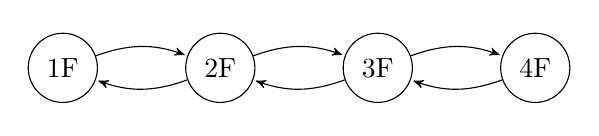
\begin{tikzpicture}[>=stealth',shorten >=1pt,auto,node distance=2cm]
  \node[state]  (q1)                {1F};
  \node[state]  (q2) [right of=q1]  {2F};
  \node[state]  (q3) [right of=q2]  {3F};
  \node[state]  (q4) [right of=q3]  {4F};

  \path[->]          (q1)  edge   [bend left=20]   node {} (q2);
  \path[->]          (q2)  edge   [bend left=20]   node {} (q1);

  \path[->]          (q2)  edge   [bend left=20]   node {} (q3);
  \path[->]          (q3)  edge   [bend left=20]   node {} (q2);

  \path[->]          (q3)  edge   [bend left=20]   node {} (q4);
  \path[->]          (q4)  edge   [bend left=20]   node {} (q3);

\end{tikzpicture}

\section{Liveness}

Consider the following elevator \textit{Spec}:
\begin{tla}
--------------------------- MODULE elevator ----------------------------
EXTENDS Integers
VARIABLES a
vars == <<a>>
TOP     == 4
BOTTOM  == 1
Init ==
    /\ a = BOTTOM
Up == 
    /\ a # TOP
    /\ a' = a + 1
Down == 
    /\ a # BOTTOM
    /\ a' = a - 1
Spec ==
  /\ Init
  /\ [][Up \/ Down]_a
=============================================================================
\end{tla}
\begin{tlatex}
\@x{}\moduleLeftDash\@xx{ {\MODULE} elevator}\moduleRightDash\@xx{}%
\@x{ {\EXTENDS} Integers}%
\@x{ {\VARIABLES} a}%
\@x{ vars \.{\defeq} {\langle} a {\rangle}}%
\@x{ TOP\@s{28.75} \.{\defeq} 4}%
\@x{ BOTTOM\@s{4.10} \.{\defeq} 1}%
\@x{ Init \.{\defeq}}%
\@x{\@s{16.4} \.{\land} a \.{=} BOTTOM}%
\@x{ Up \.{\defeq}}%
\@x{\@s{17.27} \.{\land} a \.{\neq} TOP}%
\@x{\@s{17.27} \.{\land} a \.{'} \.{=} a \.{+} 1}%
\@x{ Down \.{\defeq}}%
\@x{\@s{16.4} \.{\land} a \.{\neq} BOTTOM}%
\@x{\@s{16.4} \.{\land} a \.{'} \.{=} a \.{-} 1}%
\@x{ Spec \.{\defeq}}%
\@x{\@s{8.2} \.{\land}\@s{0.16} Init}%
\@x{\@s{8.2} \.{\land}\@s{0.16} {\Box} [ Up \.{\lor} Down ]_{ a}}%
\@x{}\bottombar\@xx{}%
\end{tlatex}

The building has a set of floors and the elevator can go either up or down. The
elevator keeps going up until it's the top floor, or keep going down until it's
the bottom floor. TLC will pass the \textit{Spec} as is.\newline

Let's introduce a liveness property. The elevator should always at least go 
to the second floor:\newline
\begin{tla}
Liveness == 
    /\ a = 1 ~> a = 2
\end{tla}
\begin{tlatex}
\@x{ Liveness \.{\defeq}}%
\@x{\@s{16.4} \.{\land} a \.{=} 1 \.{\leadsto} a \.{=} 2}%
\end{tlatex}
\newline

Running the \textit{Spec} against TLC will report a violation:

\begin{verbatim}
Error: Temporal properties were violated.
Error: The following behavior constitutes a counter-example:
State 1: <Initial predicate>
a = 1
State 2: Stuttering
\end{verbatim}

Since the \textit{Spec} permits \textit{suttering}, the state machine is allowed
to perpetually stay on 1F and \textit{never} go to 2F. This can be fixed by
introduce fairness description.

\section{Weak Fairness}

Weak fairness is defined as:\newline
\begin{equation} 
\Diamond\Box(ENABLED\langle A \rangle _v) \implies \Box\Diamond\langle A \rangle _v
\end{equation}
$ENABLED\langle A \rangle$ represents \textit{conditions required} for action A.
The above translates to: if conditions required for action A to occur is
\textit{eventually always} true, then action A will \textit{always eventually}
happen.\newline 

Without weak fairness defined, the elevator may \textit{stutter} at floor 1 and
never go to floor 2. Weak fairness states that if the conditions of an action is
\textit{eventually always} true (ie. elevator decides to stay on 1F but but
\textit{can} go up), the elevator \textit{always eventually} go up.\newline

\begin{tla}
Spec ==
  /\ Init
  /\ [][Down \/ Up]_a
  /\ WF_a(Down)
  /\ WF_a(Up)
\end{tla}
\begin{tlatex}
\@x{ Spec \.{\defeq}}%
\@x{\@s{8.2} \.{\land}\@s{0.16} Init}%
\@x{\@s{8.2} \.{\land}\@s{0.16} {\Box} [ Down \.{\lor} Up ]_{ a}}%
\@x{\@s{8.2} \.{\land}\@s{0.16} {\WF}_{ a} ( Down )}%
\@x{\@s{8.2} \.{\land}\@s{0.16} {\WF}_{ a} ( Up )}%
\end{tlatex}
\newline

Running the spec against TLC passes again. What if we want to verify the
elevator eventually always goes to the top, not just to 2F? Let's modify the
Liveness property again:\newline
\begin{tla}
Liveness == 
    /\ a = BOTTOM ~> a = TOP
\end{tla}
\begin{tlatex}
\@x{ Liveness \.{\defeq}}%
\@x{\@s{16.4} \.{\land} a \.{=} BOTTOM \.{\leadsto} a \.{=} TOP}%
\end{tlatex}
\newline

TLC now reports the following violation: 
\begin{verbatim}
Error: Temporal properties were violated.
Error: The following behavior constitutes a counter-example:
State 1: <Initial predicate>
a = 1
State 2: <Up line 10, col 5 to line 11, col 17 of module elevator>
a = 2
Back to state 1: <Down line 13, col 5 to line 14, col 17 of module elevator>
\end{verbatim}

TLC identified a case where the elevator is perpetually stuck going between 1F
and 2F, but never go to 3F. Weak fairness is no longer enough, because the the
elevator is not stuck on 2F repeatedly, but stuck going between 1F and 2F. This
is where we need strong fairness.

\section{Strong Fairness}

Strong fairness is defined as:\newline
\begin{equation} 
\Box\Diamond(ENABLED\langle A \rangle _v) \implies \Box\Diamond\langle A \rangle _v
\end{equation}
The difference between weak and strong fairness is the \textit{eventually
always} vs. \textit{always eventually}. \newline 

In weak fairness, once the state machine is stuck in a state forever, the state
machine always transition to a possible next state permitted by the spec (eg. if
the elevator is stuck on 1F but can go to 2F, it will). With strong fairness,
the elevator doesn't need to be stuck on 2F to go to 3F. If the elevator
\textit{always eventually} makes it to 2F, it \textit{eventually always} go to
3F.\newline 

Intuitively we are tempted to enable strong fairness like so: \newline
\begin{tla}
Spec ==
  /\ Init
  /\ [][Up \/ Down]_a
  /\ WF_a(Down)
  /\ SF_a(UP)
\end{tla}
\begin{tlatex}
\@x{ Spec \.{\defeq}}%
\@x{\@s{8.2} \.{\land}\@s{0.16} Init}%
\@x{\@s{8.2} \.{\land}\@s{0.16} {\Box} [ Up \.{\lor} Down ]_{ a}}%
\@x{\@s{8.2} \.{\land}\@s{0.16} {\WF}_{ a} ( Down )}%
\@x{\@s{8.2} \.{\land}\@s{0.16} {\SF}_{ a} ( UP )}%
\end{tlatex}
\newline 

However, TLC \textit{still} reports the same violation. What's going on?\newline

If we take a closer look at the enabling condition for \textit{Up}, it only
requires current floor to be not TOP. Up is \textit{always eventually} called 
even if elevator goes between 1F and 2F indefinitely (because 1F is not TOP).
What we really want is strong fairness on \textit{Up} for \textit{every floor}.
So if elevator makes to 2F once, it will eventaully go to 3F. If elevator makes
to 3F once, it will eventaully go to 4F, etc. The following is the change
required:\newline

\begin{tla}
Spec ==
  /\ Init
  /\ [][Up \/ Down]_a
  /\ WF_a(Down)
  /\ \A f \in BOTTOM..TOP-1: 
    /\ WF_a(Up /\ f = a)
\end{tla}
\begin{tlatex}
\@x{ Spec \.{\defeq}}%
\@x{\@s{8.2} \.{\land}\@s{0.16} Init}%
\@x{\@s{8.2} \.{\land}\@s{0.16} {\Box} [ Up \.{\lor} Down ]_{ a}}%
\@x{\@s{8.2} \.{\land}\@s{0.16} {\WF}_{ a} ( Down )}%
 \@x{\@s{8.2} \.{\land}\@s{0.16} \A\, f \.{\in} BOTTOM \.{\dotdot} TOP \.{-} 1
 \.{:}}%
\@x{\@s{16.4} \.{\land} {\WF}_{ a} ( Up \.{\land} f \.{=} a )}%
\end{tlatex}
\newline

Once again with this change TLC will pass.

\chapter{Reference}

\begin{thebibliography}{9}

\bibitem{}
Srikumar Subramanian
\textit{https://sriku.org/posts/fairness-in-tlaplus/}, 2015

\bibitem{}
% https://www.cds.caltech.edu/~murray/courses/afrl-sp12/L3_ltl-24Apr12.pdf
Richard M. Murray, Nok Wongpiromsarn
\textit{Linear Temporal Logic, Lecture 3}, 2012

\bibitem{backblaze}
\textit{https://www.backblaze.com/blog/cloud-storage-durability/}

\bibitem{raft}
\textit{https://raft.github.io/raft.pdf}

\bibitem{raft_tla}
\textit{https://github.com/ongardie/raft.tla}

\end{thebibliography}

\end{document}

